%%%%%%%%%%%%%%%%%%%%%%%%%%%%%%%%%%%%%%%%%%%%%%%%%%%%%%%%%%%%%%%%%%%%%%%%%%%%%%%%%%%%%%%%%%%%%%%%%%%%%%%%%%%%%%%%%%%%%%%%%%%%%%%%%%%%%%%%%%%%%%%%%%%%%%%%%%%%%%%%%%%%%%%%%%%%%%%%%%%%%%%%%%%%%%%%%%%%%%%%%%%%%%%%%%%%%%%%%%%%%%%%%%%
\chapter{The Standard Model of particle physics}

%With the formulation of a relativistic quantum field theory and of spontaneous supersymmetry breaking by the Higgs mechanism, it was made possible to explain almost all observations of particle physics up to today.
The formulation of a relativistic quantum field theory and of spontaneous symmetry breaking (SSB) by the Brout-Englert-Higgs mechanism, allowed to build a theory which is capable of explaining almost all observations of particle physics at colliders until today. %~\cite{bib:Theory:GFitter}.
This theory is known as the Standard Model (SM) of particle physics.
Its last missing piece, the Higgs boson, was found at the LHC in the year 2012~\cite{bib:Theory:CMS:HiggsObservation,bib:Theory:Atlas:HiggsObservation}.

The Standard Model is a $SU(3)_C  \times SU(2)_L \times U(1)_Y$ non-abelian gauge theory.
``After'' spontaneous symmetry breaking, its symmetries are reduced to $SU(3)_C \times U(1)_{EM}$.
All particles that were found until today are contained in it\footnote{One can argue, that the right-handed neutrino, which is proven to exist, is not contained. But as at least the left-handed neutrino is embedded, we want to ignore that for a moment.}.
Furthermore, it is able to describe three of the four fundamental forces: the strong, weak and electromagnetic force.\\

Despite its great success, there are many open questions that cannot be addressed within the Standard Model.
These ``shortcomings'' of the Standard Model will be discussed in Section~\ref{sec:Limitations}.
Before, however, a small introduction to the theory (Sections~\ref{sec:ParticleContent_SM}-\ref{sec:HiggsMechanism}) of the Standard Model is given.
It is not meant as a complete description.
For a thorough and extensive introduction, the reader is referred to~\cite{bib:SM_book_Peskin,bib:SM_book_Ryder,bib:SM_book_Griffiths}. 

\section{The particle content}
\label{sec:ParticleContent_SM}
First, it should be noted, that since the Standard Model is a quantum field theory, each type of field corresponds to a different particle type and vice versa.


The Standard Model of particle physics contains three different particle types, or three different types of fields.
First, there are the so-called ``matter particles'', which are all spin\,1/2 particles in the SM.
Second, the forces are described by spin\,1 vector bosons.
And finally, in order to give masses to all particles, the Standard Model embeds the Higgs boson, a scalar spin~0 particle.

\subsection*{Fermions in the Standard Model}
The fermionic content can be further subdivided into leptons and quarks.
In contrast to quarks, leptons are not strongly interacting, thus they only couple weakly and/or electromagnetically to other particles. 
Both, the quarks and the leptons are ordered into three different families.
Across these families, all quantum numbers are conserved.
They only differ by their mass.

All left-handed particles of each family form a $SU(2)_L$ doublet, which causes the coupling via the weak force.
The right-handed partners form $SU(2)$ singlets, thus, don't couple via the weak interaction.
As quarks carry one further quantum number, the colour, they are additionally grouped into $SU(3)_C$ triplets.


\subsection*{Vector bosons in the Standard Model}
As mentioned before, the vector bosons describe three of the four fundamental forces.
There is one gauge boson corresponding to every generator of the above mentioned gauge groups.
For $U(1)_Y$, it is the $B$-boson, for $SU(2)_L$, there are three gauge bosons $W^{1,2,3}$ and finally eight gauge bosons $G^{1...8}$ for $SU(3)_C$, which are called gluons.
As the $B$-field and the neutral $W^3$-field can mix, a change in the basis is possible ``after'' SSB and leads to the well known photon and $Z$-boson.

\subsection*{The Higgs boson}
The Higgs boson which was already predicted 50 years ago by Peter Higgs~\cite{bib:Higgs_Prediction,bib:Higgs_Prediction_2} and was found by the LHC experiments CMS and ATLAS in 2012~\cite{bib:Theory:CMS:HiggsObservation,bib:Theory:Atlas:HiggsObservation} plays a somehow extraordinary role.
This particle is a consequence of spontaneous symmetry breaking when three degrees of freedom of the Higgs field are absorbed by the $W$-and $Z$-bosons.
It is the only known fundamental scalar particle.\\


An overview of all Standard Model particles and their transformation properties are shown in Table~\ref{tab:ParticleContent_SM}.
For the $SU(3)_C$ and $SU(2)_L$ gauge groups, the corresponding representations are given for each of the particle types.
For the $U(1)_Y$ gauge group, the corresponding quantum number, the so-called hypercharge, is depicted.
If particles transform as singlets under $SU(2)_L$ or $SU(3)_C$, they don't couple via the corresponding force.
The hypercharges $Y$ are determined by $Q=Y+I_3$, where $Q$ is the electric charge and $I_3$ is the third component of the weak isospin with $I^a = \sigma^a/2$, $\sigma^a$ being the Pauli matrices. 

\renewcommand{\arraystretch}{1.4}
\begin{table}[!h]
\centering
\caption{All particles contained in the Standard Model and their transformation properties under $SU(3)_C  \times SU(2)_L \times U(1)_Y$. 
         For the gauge groups $SU(3)_C$ and $SU(2)_L$, the representations are listed whereas for $U(1)_Y$ the hypercharge is given.}
\label{tab:ParticleContent_SM}
\makebox[0.99\textwidth]{
\begin{tabular}{llll}
\multicolumn{4}{c}{} \\
\toprule
                              & $SU(3)_C$         & $SU(2)_L$    & $U(1)_Y$            \\
\midrule
Fermions:                     &                   &              &                     \\
\midrule
$\left( \nu_L , e_L \right)^T$ & \textbf{1}         & \textbf{2}            & $-1$ \\
$e_R$                          & \textbf{1}        & \textbf{1}             & $-2$ \\ 
$\left( u_L , d_L \right)^T$   & \textbf{3}         & \textbf{2}              & $+\frac{1}{3}$ \\
$u_R$                          & \textbf{3}        & \textbf{1}             & $+\frac{4}{3}$ \\ 
$d_R$                          & \textbf{3}        & \textbf{1}             & $-\frac{2}{3}$ \\ 
\midrule
 Vector bosons:                &        &          &             \\
\midrule
$B_{\mu}$                       & \textbf{1}        & \textbf{1}             & 0 \\ 
$W_{\mu}^{a}$                    & \textbf{1}        & \textbf{3}             & 0 \\ 
$G_{\mu}^{a}$                    & \textbf{8}        & \textbf{1}             & 0 \\ 
\midrule

Higgs boson: $H$            &  \textbf{1}        & \textbf{2}             & $-1$ \\ 
\bottomrule
\multicolumn{4}{c}{}
\end{tabular}}
\end{table}  


\section{The Lagrangian density}
In particle physics, the dynamics of a particle system is described by the Lagrangian density.
The Lagrangian density of the Standard Model is the most general set of Lagrangian terms, that are renormalisable and contain all up to date known particles as well as the above mentioned symmetries.
The full SM Lagrangian density reads as follows:
\begin{equation}
\begin{split}
 \mathcal{L} =& \left( D_{\mu} \Phi \right)^{\dagger} \left( D^{\mu} \Phi \right) -\mu^2\Phi^{\dagger} \Phi -\frac{\lambda}{4} \left( \Phi^{\dagger} \Phi \right)^2\\
 & + \bar{L}^L_i i \slashed{D} L^{L}_i + \bar{e}^{R}_i i \slashed{D} e^{R}_i +  \bar{Q}^L_{i\,b} i \slashed{D} Q^L_{i\,b} + \bar{u}^{R}_{i\,b} i \slashed{D} u^{R}_{i\,b} +
\bar{d}^{R}_{i\,b} i \slashed{D} d^{R}_{i\,b}\\
& - \left( Y^e_{ij} \bar{L}^L_i \Phi e^R_j + Y^u_{ij} \bar{Q}^L_{i\,b} \Phi^c u^R_{j\,b} + Y^d_{ij} \bar{Q}^L_{i\,b} \Phi d^R_{j\,b} + h.c. \right)\\
& - \frac{1}{4} \left( B_{\mu\nu}  B^{\mu\nu} +  W^a_{\mu\nu} W^{a\,\mu\nu} +  G^a_{\mu\nu} G^{a\,\mu\nu}    \right),
\end{split}
\label{eq:LagrangianDensity}
\end{equation}
with $\slashed{D} = \gamma_{\mu} D^{\mu}$ and the covariant derivative $D^{\mu}=\partial^{\mu} + i g' Y_W B^{\mu} - i g C_1  I^a W_a^{\mu}  - i g_S C_2 T^a G_a^{\mu}$ including the three gauge couplings $g$, $g'$ and $g_S$.
$I^a$ and $T^a$ denote the generators of the $SU(2)_L$ and $SU(3)_C$, respectively.
They are connected to the three Pauli matrices and the eight Gell-Mann matrices by $I^a = \frac{\sigma^a}{2}$ and $T^a = \frac{\lambda^a}{2}$.
The sum of the hypercharge $Y_W$ and the third component of the weak isospin yields the electrical charge $Q=Y_W + I_3$.
Furthermore, it is $C_1=1 $ for doublets and $C_1=0$ for singlets under $SU(2)_L$, $C_2=1$ for triplets and $C_2=0 $ for singlets under $SU(3)_C$.  

The first line in Eq.~\eqref{eq:LagrangianDensity} corresponds to the kinetic term of the Higgs field and its potential.
Via this Higgs field, it is possible to give masses to the $Z$-and $W^{\pm}$-bosons as well as the fermions.
This will be explained in detail in the following Section~\ref{sec:HiggsMechanism}.
The second line describes the kinetic terms of the leptons and quarks.
The index $i$ represents the three different families ($i=1,2,3$).
Since they are spin\,1/2 particles, they can be described with the help of Dirac spinors.
The left-handed leptons and quarks are described as $SU(2)_L$ doublets, $L_I^L = \left( \nu_{e\,L},e_L\right)_i$, $Q_I^L = \left( u_{L},d_L\right)_i$,  the right-handed as singlets under $SU(2)_L$ $e_i^R$, $u_i^R$, $d_i^R$.
Quarks carry a further quantum number, the colour, which is indicated by the index $b$ with $b=1,2,3$.
Quarks transform as triplets under the $SU(3)_C$ gauge group.
The third line contains the interaction terms between the fermions and the Higgs boson, called Yukawa interactions.
After SSB, these terms lead to the fermion mass terms as can be seen later.
The last line correspond to the kinetic terms of the gauge fields.
These are connected to the field strength tensors by
\begin{equation}
 \begin{split}
  B^{\mu\nu} \equiv &\ \partial^{\mu} B^{\nu} - \partial^{\nu} B^{\mu}\\  
  W^{\mu\nu} \equiv &\ \partial^{\mu} W^{\nu} - \partial^{\nu} W^{\mu} -i g \left[W^{\mu}, W^{\nu} \right]\\
             =& \left( \partial^{\mu} W_i^{\nu} -\partial^{\nu} W_i^{\mu} + g\, \epsilon_{ijk} W_j^{\mu} W_k^{\nu}  \right) \frac{\sigma_i}{2} \equiv \frac{\sigma_i}{2} W_a^{\mu\nu}\\
  G^{\mu\nu} \equiv &\ \partial^{\mu} G^{\nu} - \partial^{\nu} G^{\mu} - i g_S \left[G^{\mu}, G^{\nu} \right] \\
            =& \left( \partial^{\mu} G_a^{\nu} -\partial^{\nu} G_a^{\mu} + g_S f_{abc} G_b^{\mu} G_b^{\nu}  \right) \frac{\lambda_a}{2} \equiv \frac{\lambda_a}{2} G_a^{\mu\nu}.\\
 \end{split}
\end{equation}
The factors $\epsilon_{ijk}$ and $f_{abc}$ are the structure constants of the corresponding Lie groups.
The notation implies a summation over all indices that appear twice.

\section{The Brout-Englert-Higgs mechanism}
\label{sec:HiggsMechanism}
An essential ingredient of the Standard Model is the Brout-Englert-Higgs mechanism (BEH mechanism), earlier also called Higgs mechanism.
It was developed by Peter Higgs, Robert Brout and Fran\c{c}ois Englert in the 1960s~\cite{bib:HiggsMechanism_Brout_Englert,bib:Higgs_Prediction,bib:Higgs_Prediction_2,bib:HiggsMechanism_Guralnik_Hagen_Kibble,bib:HiggsMechanism_Higgs_1966,bib:HiggsMechanism_Kibble_1967}. 
Based on work from Sheldon Glashow~\cite{bib:HiggsMechanism_Glashow_1961}, the BEH mechanism was later applied to a $SU(2) \times U(1)$ gauge theory by Steven Weinberg and Abdus Salam~\cite{bib:HiggsMechanism_Weinberg_1967,bib:HiggsMechanism_Salam_1968}.
By this, a renormalisable theory of the weak and the electromagnetic interactions was born.
%Together with the theory of strong interaction, quantum chromodynamics, the formulation of the Standard Model was thus complete by the early 1970s.

\subsection*{Mass terms of the gauge bosons}
Due to the BEH mechanism, it is possible to give masses to the $W^{\pm}$-and Z-bosons.
A scalar field $\Phi$ (Higgs field) is required, which has a non-zero vacuum expectation value.
This is possible, if the mass parameter $\mu$ in front of the bilinear term in line one of Eq.~\eqref{eq:LagrangianDensity} is smaller than zero and $\lambda>0$ at the same time.

The resulting potential of the Higgs field is then the famous ``Mexican hat'' potential.
Expanding the Lagrangian density around the minimum of $\Phi = \left( 0,v \right)$, the gauge symmetries of $SU(2)_L \times U(1)_Y$ are spontaneously broken and only the electrical charge conserving symmetry $U(1)_{EM}$ remains.
After a unitary transformation, three of the four degrees of freedom of the Higgs field are absorbed by the gauge fields.
Thus, ``after'' SSB, the part of the Lagrangian containing the scalar field is as follows
\begin{equation}
\begin{split}
\mathcal{L}_{\text{Higgs}} =& \frac{1}{2} \left( \partial_{\mu} h^0 \right)^{\dagger} \left( \partial^{\mu} h^0 \right) - \mu^2 \left(h^0\right)^2 + \frac{1}{2} v^2 g^2 W_{\mu}^- W^{+\,\mu}
                    + \frac{1}{4} v^2 \left(g^2 + g'^2  \right)  Z_{\mu} Z^{\mu}\\
  &+ \text{interaction terms}
\end{split}
\label{eq:LHiggs}
\end{equation}
One kinetic and one mass term for one of the degrees of freedom of the Higgs fields remains, which is the Higgs boson ($h^0$).
Furthermore, three of the four gauge bosons acquire a mass.
The remaining gauge boson, the photon, remains massless because of the conserved $U(1)_{EM}$ gauge symmetry.

The mass eigenstates of the gauge bosons in Eq.~\eqref{eq:LHiggs} are obviously different to the interaction eigenstates in Eq.~\eqref{eq:LagrangianDensity}.
The diagonalisation of the neutral mass matrices is described by the Weinberg angle $\theta_W$
\begin{equation}
 \begin{pmatrix} A_{\mu} \\ Z_{\mu} \end{pmatrix} = 
   \begin{pmatrix} \cos \theta_W & - \sin \theta_W \\ \sin \theta_W  & \cos \theta_W \end{pmatrix} \begin{pmatrix} B_{\mu} \\ W^3_{\mu} \end{pmatrix}.
\end{equation}
For the charged gauge bosons, the relation between $W_{1,2}$ and $W^{\pm}$ is the following
\begin{equation}
 W_{\mu}^{\pm}= \frac{1}{\sqrt{2}} \left[ W_{\mu}^1 \mp W_{\mu}^2  \right].
\end{equation}
Consequently, the masses of the gauge bosons are the following (with $\sin{\theta_W} = \frac{g'}{\sqrt{g^2 + g'^2}}$)
\begin{equation}
 \begin{split}
  M_H =\,&  \sqrt{2} \mu\\
  M_W =\,& \frac{g}{\sqrt{2}}\, v\\
  M_Z =\,& \frac{1}{\sqrt{2}}\, v \sqrt{g^2 + g'^2}\\
  M_{\gamma} =\,& 0.
 \end{split}
\end{equation}
The first direct observation of the $Z$-and $W^{\pm}$-bosons was made in $p\overline{p}$-collisions in the year 1983 at the Super Proton Synchrotron (SPS) at CERN~\cite{bib:W_discovery,bib:Z_discovery}.
The experimental values of the masses are $m_{Z}=91.1876\pm0.0021\gev$ and $m_{W^{\pm}}=80.385\pm0.015\gev$~\cite{bib:PDG_2014}.
Finally, as mentioned several times before, the Higgs boson was found at the LHC in the year 2012~\cite{bib:Theory:CMS:HiggsObservation,bib:Theory:Atlas:HiggsObservation}.
The mass is measured to $m_{h^0}=125.09 \pm 0.21\text{(stat.)} \pm 0.11\text{(sys.)}\gev$~\cite{bib:HiggsMass}.

\subsection*{Mass terms of the fermions}
Fermion mass terms cannot be easily inserted into the Lagrangian density in Eq.~\eqref{eq:LagrangianDensity}, since they would violate the imposed gauge symmetries.
With the help of the BEH mechanism it is possible to generate fermion mass terms via the Yukawa interaction terms (line three of Eq.~\eqref{eq:LagrangianDensity}).
After spontaneous symmetry breaking, the Yukawa interactions lead to the following mass terms (colour indices are suppressed)
\begin{equation}
 \begin{split}
  \mathcal{L}_{\text{Yukawa}} = & - \left( Y^e_{ij}\, v\, \bar{e}^L_i  e^R_j + Y^u_{ij}\, v\, \bar{u}^L_i  u^R_j 
+ Y^d_{ij}\, v\, \bar{d}^L_i  d^R_j + h.c. \right) \\
    &+ \text{interaction terms}
 \end{split}
\end{equation}
The fermion masses are thus described by the following mass matrices
\begin{align}
 M_{ij}^e = Y_{ij}^e \, v && M_{ij}^u =  Y_{ij}^u \, v && M_{ij}^d =  Y_{ij}^d \, v 
\end{align}
Since the Standard Model does not contain right-handed neutrinos, there are no gauge invariant Yukawa interactions, that could produce mass terms for neutrinos.

%As said before, the Standard Model contains nine different massive fermions, three leptons and six quarks.
%The leptonic masses are measured to the following values~\cite{bib:PDG_2014}
%\begin{equation}
%\begin{split}
%m_e     &= 0.510998929 \pm 0.000000011\mev  \\
%m_{\mu}  &= 105.6583715 \pm 0.0000035\mev  \\
%m_{\tau} &=  1776.82 \pm 0.16 \mev 
%\end{split}
%\end{equation}

%Since quarks cannot exists freely, because of the strong interaction, the definition of mass is a problematic concept for quarks.
%In the $\overline{MS}$ scheme, the values are the following~\cite{bib:PDG_2014}
%\begin{equation}
%\begin{split}
%m_u     &=  2.3^{+0.7}_{-0.5}\mev   \\
%m_d     &=  4.8^{+0.5}_{-0.3}\mev   \\
%m_s     &=  95 \pm 5 \mev        \\
%m_c     &=  1.275 \pm 0.025 \gev \\
%m_b     &=  4.18 \pm 0.03 \gev   \\
%m_t     &=  160^{+5}_{-4} \gev.
%\end{split}
%\end{equation}
%The last fermion that was discovered in the year xxx is the top quark, 

\section{Limitations of the Standard Model}
\label{sec:Limitations}
Despite the great success of the Standard Model, there remain observations and theoretical considerations that cannot be answered within the SM.
In the following, the most important of such ``limitations'' shall be reviewed.\\

First of all, the Standard Model suffers from the so-called hierarchy problem.
It is caused by the occurrence of quadratic divergencies in the calculation of the Higgs mass.
The appearance of infinities is not uncommon in higher order calculations and happens for all particles. 
Still, for scalar particles the infinite term is quadratically divergent, which makes a huge difference compared to the logarithmic divergencies for fermion self-energies. 
When considering the Standard Model valid up to the Planck scale, an extraordinary fine-tuning would be needed to cancel a large bare mass with large counter terms 
\begin{equation}
 m^{\text{ren}\,2}_{h^0} = m_{h^0}^{\text{bare}\,2} + \Delta m^2_{h^0}
\end{equation}
to end up with a Higgs mass of about 125\gev.
Thus, this renormalisation procedure, even if mathematically possible, is regarded as highly unnatural.
This raises the question why the Higgs mass is so small, despite the presence of such massive radiative corrections to the bare bass.
A formulation of naturalness was given by t'Hooft in 1977~\cite{bib:Naturalness_tHooft}. 
He stated, that a small parameter can only be regarded natural, if the symmetries of the theory are enhanced by setting this parameter to zero.
In the Standard Model, though, there is no enhancement of the symmetries of the Lagrangian by setting $\mu=0$.
Thus, the small mass of the Higgs boson compared to the Planck scale is considered as highly unnatural.

A further and probably the most striking shortcoming of the Standard Model is the missing fourth fundamental force, the gravitational force.
Within the SM, it is not possible to add renormalisable terms, that can describe the gravitational force.
Although, gravity is not important for particle physics at energies that are accessible at current particle colliders (it only becomes important at the Planck scale $\sim 10^{19}\gev$), the fact that it cannot be embedded into the Standard Model leads to an understanding of the SM as an effective theory, only valid for low energies.
Thus, it is obviously not an ultimate theory and something must be beyond.

Furthermore, in particle physics there is always the wish to describe nature with a theory as simple as possible.
This usually implies the effort to embed the Standard Model into a higher symmetry group.
To achieve a simplification by unifying the three fundamental forces is usually done within so-called Grand-Unified-Theories (GUTs).
Calculating the running of the coupling constants in the Standard Model, the couplings seem to meet at a scale of $M_{\text{GUT}} \sim 10^{15}\gev$.
Unfortunately, they don't meet exactly.
Therefore, a unification is not achievable in the Standard Model under the assumption that there are no new particles up to the GUT scale.


Finally, there is experimental evidence that cannot be explained within the Standard Model.
Astrophysical observations suggest that there is a large amount of Dark Matter (DM) in the universe, that cannot be explained with the particle content of the Standard Model.
Measurements of the velocity curves of galaxies, \eg M33~\cite{bib:DM:RotationCurves} show discrepancies between the observed velocities and the velocities predicted from visible matter.
Furthermore, the measurement of the cosmic microwave background~\cite{bib:Planck_2015} together with type Ia supernovae measurements~\cite{bib:Supernovae} hint at a large DM fraction.
The share of non-visible matter to the total amount of matter in the universe is estimated to be $\sim84\%$~\cite{bib:Planck_2015}.
Unfortunately, there is no suitable (only weakly interacting) candidate within the SM, that can make up the full DM contribution.\\

In the following Chapter~\ref{ch:Supersymmetry}, a theory is introduced, that can address most of the above mentioned problems.
This theory is called supersymmetry.


\chapter{Supersymmetry}
\label{ch:Supersymmetry}

As noted in the last chapter, the Higgs boson mass suffers from quadratic divergencies through radiative corrections.
The reason for the quadratic divergencies is due to the fact, that the Lagrangian density does not contain further symmetries for $\mu\rightarrow 0 $.
This behaviour is typical for scalar particles.
For fermions, on the other hand, there is a further symmetry for $m_f=0$. 
The Lagrangian density becomes invariant under chiral transformations of the form $\Psi \rightarrow e^{i\vec{\alpha}\frac{\vec{\sigma}}{2} \gamma_5} \Psi$.
Although the mass terms of the fermions break this symmetry, it protects the fermions against large radiative corrections.

Due to these considerations, it seems natural to transfer the mechanism of protecting fermion masses by a chiral symmetry to scalar masses as well.
This can only be done by connecting fermions with bosons and vice versa.
In the 1970s, exactly this linking between the different particle types was achieved.
A work from Golfand and Likhtman in the year 1971 stated that an extension of the Poincar\'e  algebra is possible via fermionic generators~\cite{bib:Golfand_Likhtman_1971}.
R.~Haag, J.~Lopuszanski and M.~Sohnius finalised these considerations by showing that with the help of fermionic generators a connection between space-time symmetries and internal symmetries is possible~\cite{bib:Haag_1974}.
The extensions of a symmetry group by fermionic generators is called supersymmetry (SUSY).
These were the foundation of supersymmetric theories.\\

In the following, the most important aspects of supersymmetric theories are discussed.
For a detailed introduction the reader is referred to~\cite{bib:Drees_1996,bib:Aitchison_2005,bib:Drees_2004}.

In the subsequent sections, the description is restricted to the case of $\mathcal{N}=1$ supersymmetry, \ie there is only one supersymmetric generator and thus only one supersymmetric partner for every particle.
A supersymmetric transformation transfers every bosonic state into a fermionic state and vice versa  
\begin{equation}
\begin{split}
 Q\, |\text{boson}\rangle  &= |\text{fermion}\rangle\\ 
 Q\, |\text{fermion}\rangle  &= |\text{boson}\rangle.
\end{split}
\end{equation}
The most important (anti-) commutation relations for SUSY algebra with fermionic generators Q are
\begin{align}
\label{eq:SUSYal}
 \{Q_{\alpha},Q_{\beta} \} &=  \{Q^{\dagger}_{\dot{\alpha}},Q^{\dagger}_{\dot{\beta}} \} = 0,\nonumber \\
   [Q_{\alpha} , P_{\mu}] &=  [Q^{\dagger}_{\dot{\alpha}}, P_{\mu}] = 0 ,\\
\{Q_{\alpha},  Q^{\dagger}_{\dot{\alpha}}\} &= 2 \sigma_{\alpha\dot{\alpha}}^{\mu} P_{\mu} \nonumber.
\end{align}
Here, $P_{\mu}$ denotes the four component generator of translations and $\sigma^{\mu} = \left( \mathbbm{1}, \sigma_i  \right)$ with the Pauli matrices $\sigma_i$.
From the second relation in~\eqref{eq:SUSYal} follows
\begin{align}
\label{eq:Massen}
 [Q_{\alpha} , P^2] &=  [Q^{\dagger}_{\dot{\alpha}}, P^2] = 0.
\end{align}
Equation~\ref{eq:Massen} implies, that particles that are transformed into each other with the generator $Q$ need to have the same eigenvalues of $P^2$, thus, also the same masses.
This obviously imposes a problem, since no ``scalar electron'' was ever found with a mass of 0.51\mev.
Therefore, SUSY must be broken.
There are many ideas how the breaking can actually happen.
However, since up to now, only little is known about the breaking mechanism, usually further terms which break SUSY explicitly, are added by hand to the Lagrangian density.
These terms can parametrise SUSY breaking without any knowledge about the breaking mechanism.
One condition is however imposed on the supersymmetry breaking terms: they should not spoil the naturalness of the new theory, \ie no new quadratic divergencies shall occur due to these terms.
Therefore, they are called soft-breaking terms.
How they actually look, will be explained in the Section~\ref{sec:MSSM}.\\

Finally, it shall be discussed how a supersymmetric extension of the Standard Model can give possible answers to the shortcomings of the Standard Model, discussed in Section~\ref{sec:Limitations}.

Radiative corrections by fermions always have a factor $-1$ compared to bosonic corrections.
Thus, calculating radiative corrections of the Higgs boson mass in a supersymmetric theory leads in addition to the corrections by SM particles to further corrections by SUSY particles.
If SUSY were exact, the quadratic divergencies $\Delta m^2_{h^0}$ would exactly cancel. 
However, as argued, SUSY must be broken.
The cancellation of quadratic divergencies can therefore only be assured, if the breaking is ``soft'', \ie only logarithmic divergencies remain.
%To avoid a new source of fine-tuning, the soft-breaking parameters should be of the order $M_{\rm soft} \sim 100\gev - 1000\gev$.

Embedding gravity into a four dimensional quantum field theory proves difficult because of the non-renormalisability of the resulting theory.
A possible answer, beyond quantum field theory, are string theories~\cite{bib:Strings_1974}, where the existence of a fundamental length - that of the strings - regularises the ultraviolet behaviour and allows for a quantum description of objects in curved space.
Yet, the only known procedure to incorporate fermions within a string Lagrangian density consists in adding supersymmetry as a condition. 
Supersymmetry thus appears as a fundamental ingredient for a description of quantum gravity. % and it might be partially preserved at low energy (close to the TeV scale).

%It is not possible to implement gravity within a renormalisable $\mathcal{N}=1$ supersymmetric extension of the Standard Model.
%However, so-called string theories are able to incorporate quantum gravity and, furthermore, string theories that allow for bosons and fermions are based on supersymmetry.
%Therefore, supersymmetry is considered as a crucial ingredient for the description of a quantum field theory of gravity.


The renormalisation group equations change under a supersymmetric extension of the Standard Model.
By this, a unification of the gauge couplings at a GUT scale of about $10^{16}\gev$ is possible, as can be seen in Fig.~\ref{fig:Unification}.
It can be nicely seen, that all three gauge couplings cross each other within the uncertainties.
\begin{figure}[!t]
  \centering
      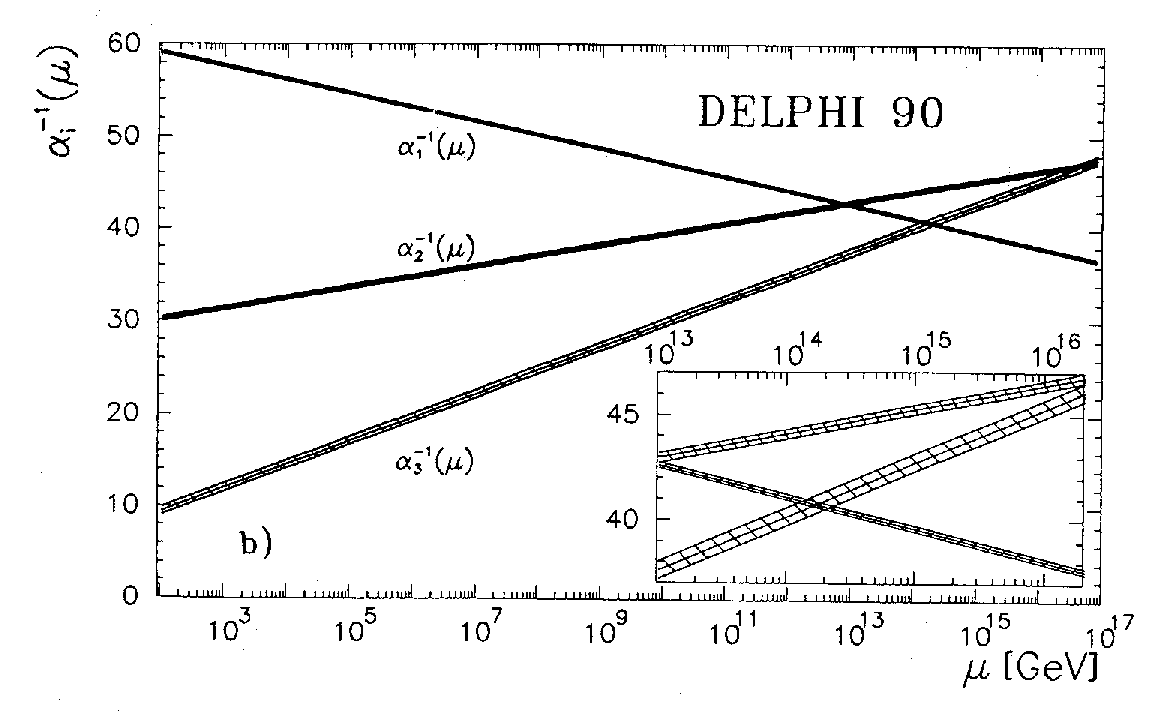
\includegraphics[width=0.49\textwidth]{figures/theory/running_couplings_SM}
      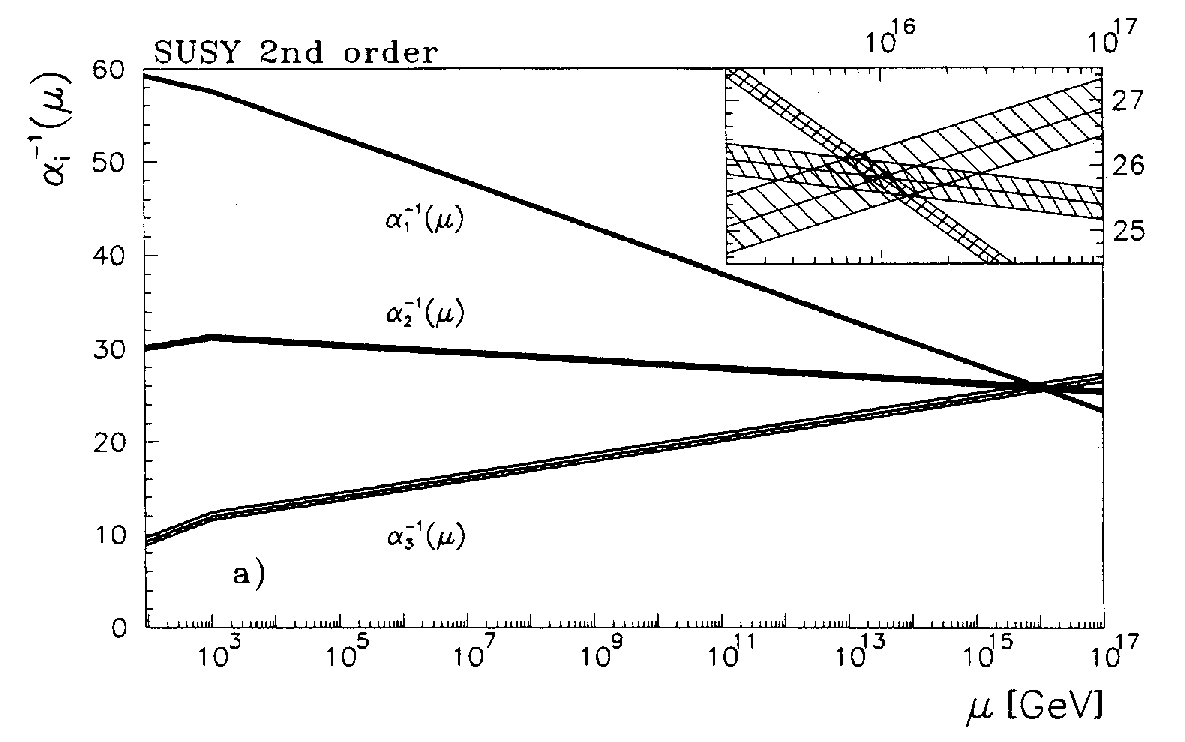
\includegraphics[width=0.49\textwidth]{figures/theory/running_couplings_MSSM}
  \caption{The running of the gauge couplings in the Standard Model (left) and in the minimal supersymmetric extension of the SM (right). Taken from~\cite{bib:Unification}.}  
  \label{fig:Unification}
\end{figure}

Besides these arguments, SUSY can also provide an answer to the problem of non-visible matter in the universe.
If the conservation of the so-called R-parity is required, the lightest supersymmetric particle (LSP) is stable.
If this particle is only weakly interacting, it can serve as a good candidate to explain fully or partially the sources of the relic density. 
R-parity is a multiplicative quantum number with 
\begin{equation}
\begin{aligned}
P_R & =  1 \qquad &&\text{SM particles}\\
P_R & = -1 &&\text{SUSY particles}.
\end{aligned}
\end{equation}
If R-parity is conserved, only terms are allowed in the Lagrangian density, that contain an even number of supersymmetric particles.
Therefore, no single SUSY particle can decay into only SM particles and thus, the LSP is stable.
The following discussions are restricted to R-parity conserving supersymmetric models.



\section{The MSSM}
\label{sec:MSSM}
The supersymmetric extension of the Standard Model with a minimal particle content is called the Minimal Supersymmetric Standard Model (MSSM).
In the following section, the particle content of the MSSM is introduced.

\subsection{The particle content of the MSSM}
In $\mathcal{N}=1$ supersymmetry, every SM particle has exactly one supersymmetric partner particle, which leads to a doubling of the particle content in the MSSM with respect to the SM\footnote{The supersymmetric partner particles of the fermions are called sfermions, whereas the partner particles of the gauge (Higgs) bosons are referred to as gauginos (higgsinos).}.
Additionally, it is necessary to introduce a second Higgs doublet to ensure the holomorphicity of the superpotential in the presence of mass terms for the up-type particles.
Furthermore, the MSSM only stays free from anomalies if there is a further Higgs doublet~\cite{bib:SUSYPrimer}.
This leads to the fact, that in the MSSM, there are five Higgs bosons instead of only one as in the SM.

\renewcommand{\arraystretch}{1.5}
\begin{table}[!b]
\centering
\caption{Chiral supermultiplets in the MSSM.}
\label{tab:chiral_multiplets}
\makebox[0.99\textwidth]{
\begin{tabular}{l|c|c|c}
\multicolumn{4}{c}{} \\
\toprule
                     &   spin 0                                     & spin $\frac{1}{2}$              & $SU(3)_C,\ SU(2)_L,\ U(1)_Y$\\ 
\midrule
   squarks/quarks    & $\left(\tilde{u}_L,\tilde{d}_L \right)$      & $\left(u_L,d_L\right)$           & $\mathbf{3},\ \mathbf{2},\ +\frac{1}{3}$\\ \cline{2-4}  
                     & $\tilde{\bar{u}}_L = \tilde{u}_R^{\dagger} $   & $\bar{u}_L = (u_R)^c$            & $\mathbf{\bar{3}},\ \mathbf{1},\ -\frac{4}{3}$\\ \cline{2-4}  
                     & $\tilde{\bar{d}}_L = \tilde{d}_R^{\dagger}$    & $\bar{d}_L = (d_R)^c$            & $\mathbf{\bar{3}},\ \mathbf{1},\ +\frac{2}{3}$\\ 
\midrule
   sleptons/leptons  & $\left(\tilde{\nu}_{eL},\tilde{e}_L\right)$   & $\left(\nu_{eL},e_L\right)$      & $\mathbf{1},\ \mathbf{2},\ -1$\\ \cline{2-4} 
                     & $\tilde{\bar{e}}_L = \tilde{e}_R^{\dagger}$    & $\bar{e}_L = (e_R)^c$            & $\mathbf{\bar{1}},\ \mathbf{1},\ +2$\\ 
\midrule
   Higgs/higgsinos   & $\left(H_u^+,H_u^0\right)$        & $\left(\tilde{H}_u^+,\tilde{H}_u^0\right)$   & $\mathbf{1},\ \mathbf{2},\ +1$\\ \cline{2-4}
                     & $\left(H_d^0,H_d^-\right)$        & $\left(\tilde{H}_d^0,\tilde{H}_d^-\right)$   & $\mathbf{1},\ \mathbf{2},\ -1$ \\ 
\bottomrule
\multicolumn{4}{c}{} 
\end{tabular}}
\end{table}  
\renewcommand{\arraystretch}{1.5}
\begin{table}[!t]
\centering
\caption{Vector supermultiplets in the MSSM.}
\label{tab:vector_multiplets}
\makebox[0.99\textwidth]{
\begin{tabular}{l|c|c|c}
\multicolumn{4}{c}{} \\
\toprule
                      &   spin $\frac{1}{2}$                                  & spin 1                 & $SU(3)_C,\ SU(2)_L,\ U(1)_Y$\\ 
\midrule
   gluinos/gluons     & $\tilde{g}$                       & $g$                 & $\mathbf{8},\ \mathbf{1},\ 0$\\ 
\midrule
   winos/$W$-bosons   & $\tilde{W}^{\pm},\ \tilde{W}^0$  & $W^{\pm},\ W^0$     & $\mathbf{1},\ \mathbf{3},\ 0$\\
\midrule
   bino/$B$-boson     & $\tilde{B}$                      & $B$                 & $\mathbf{1},\ \mathbf{1},\ 0$ \\  
\bottomrule
\multicolumn{4}{c}{}
\end{tabular}}
\end{table} 
In supersymmetry, all particles and their partner particles are described by so-called supermultiplets.
Since the generators of the gauge group commute with the generators of supersymmetry, all particles within one supermultiplet have same quantum numbers, besides the spin.
In a renormalisable theory, there are two different types of supermultiplets: chiral multiplets, which contain a two-component Weyl spinor describing the fermionic degrees of freedom and a complex scalar field for the bosonic degrees of freedom; vector multiplets containing a vector field and a two-component Weyl spinor.
The complete particle content of the MSSM is depicted in Tables~\ref{tab:chiral_multiplets} and~\ref{tab:vector_multiplets}. 
Since in supersymmetric theories only left-handed Weyl spinors appear in the Lagrangian density, the right-handed particles are described as charge conjugated spinors of the left-handed spinors.


\subsection{The Lagrangian density of the MSSM}
\label{sec:Lagrange_MSSM}
In the following, only the most important parts of the MSSM Lagrangian density will be described.
For a complete description of the Lagrangian density, the reader is again referred to~\cite{bib:Drees_2004}.

\subsubsection*{The superpotential}
The superpotential of the MSSM contains the self interaction terms of the Higgs bosons and generates the interaction terms of the Higgs bosons with the fermions and their superpartners.
As already noted, it is very common to assume R-parity conservation.
Hence, no terms appear in the Lagrangian that would violate lepton or baryon number conservation and the lightest supersymmetric particle is stable.
Thus, all possible terms are
\begin{equation}
\label{eq:SPMSSM}
 W_{\text{MSSM}} = \mu H_u \cdot H_d - Y_u^{ij} H_u \cdot Q_L^i u_R^{c\,j} + Y_d^{ij} H_d \cdot Q_L^i d_R^{\,c\,j} + Y_e^{ij} H_d \cdot L_L^i e_R^{c\,j},
\end{equation}
with the dot product defined as in~\cite{bib:Aitchison_2005} 
\begin{equation}
 A \cdot B = \epsilon^{\alpha\beta} A_{\alpha} B_{\beta} = A_1 B_2 - A_2 B_1.
\end{equation}

\subsubsection*{The soft-breaking Lagrangian density}
Since supersymmetry is broken, explicit SUSY breaking terms are added to the Lagrangian density.
In order not to introduce new sources of quadratic divergencies, only bilinear and trilinear terms appear in the soft-breaking Lagrangian
\begin{equation}
 \begin{split}
  - \mathcal{L}^{MSSM}_{soft} =\,& m_{H_u}^2 H_u^{\dagger} \cdot H_u +m_{H_d}^2 H_d^{\dagger} \cdot H_d + \left(B\mu\, H_u \cdot H_d + h.c.\right) \\
  & + m_{\tilde{Q}\,ij}^2 \tilde{Q}_{L\,i}^{\dagger} \cdot \tilde{Q}_{L\,j}+ m_{\tilde{u}\,ij}^2 \tilde{u}_{R\,i}^{c\,\dagger} \cdot \tilde{u}_{R\,j}^c
+ m_{\tilde{d}\,ij}^2 \tilde{d}_{R\,i}^{\,c\,\dagger} \cdot \tilde{d}_{R\,j}^{\,c}\\
& + m_{\tilde{L}\,ij}^2 \tilde{L}_{L\,i}^{\dagger} \cdot \tilde{L}_{L\,j}+ m_{\tilde{e}\,ij}^2 \tilde{e}_{R\,i}^{\,c\,\dagger} \cdot \tilde{e}_{R\,j}^{\,c}\\
& +\left(- \left( A_u Y_u \right)_{ij} H_u \cdot \tilde{Q}_{L\,i} \tilde{u}_{R\,j}^c +\left( A_d Y_d \right)_{ij} H_d \cdot \tilde{Q}_{L\,i} \tilde{d}_{R\,j}^{\,c} \right.\\
& \left. +\left( A_e Y_e \right)_{ij} H_d \cdot \tilde{L}_{L\,i} \tilde{e}_{R\,j}^{\,c} + h.c. \right)\\
& + \left(M_1 \tilde{B} \tilde{B} + M_2 \tilde{W}_a \tilde{W}_a + M_3 \tilde{g}_i \tilde{g}_i + h.c \right)
 \end{split}
\label{eq:SoftTerms}
\end{equation}
The first line contains mass terms for the Higgs bosons, the second and third line for the sfermions.
In the fourth and fifth line the trilinear couplings between the Higgs bosons and the sfermions appear.
Finally, the last line gives rise to mass terms for the gauginos (gluinos, winos, bino).

Because of the soft-breaking terms, the MSSM contains more than 100 free parameters.
Constraining the MSSM is thus a difficult task and usually in experimental particle physics, constrained versions of the MSSM or assumptions at the GUT scale are used to report the impact of searches on SUSY. 
In the following a short introduction of the phenomenological MSSM is given.
With its reduced parameter space, it allows to elaborate on long-lived particles in the MSSM in a much easier way.

\subsection{The phenomenological MSSM}
\label{subsec:pMSSM}
The phenomenological MSSM (pMSSM) imposes constraints that are reasonable in the sense that the pMSSM fulfils current observations and still keeps the phenomenological variety of the MSSM~\cite{bib:pMSSM}.
The following assumptions are imposed (in~\cite{bib:pMSSM} more detailed information about these assumptions can be found):
\begin{itemize}
\item No new sources of CP violation,
\item No flavour changing neutral currents,
\item First and second generation universality.
\end{itemize}
These assumption reduce the number of SUSY parameters to only 19.
The remaining free parameters are the following:
\begin{itemize}
\item $\tan \beta$ (the ratio of the vacuum expectation values of the two Higgs doublets)
\item $M_A$ (the mass of the pseudo-scalar Higgs boson)  
\item $\mu$ (the Higgs mass parameter)
\item $M_1$,$M_2$,$M_3$ (bino, wino and gluino mass parameters, respectively)
\item $m_{\tilde{q}}$, $m_{\tilde{l}}$, $m_{\tilde{u}}$, $m_{\tilde{d}}$ and $m_{\tilde{e}}$ (the first and second generation mass parameters)
\item  $m_{\tilde{Q}}$, $m_{\tilde{L}}$, $m_{\tilde{t}}$, $m_{\tilde{b}}$ and $m_{\tilde{\tau}}$ (the third generation mass parameters)
\item $A_t$, $A_b$ and $A_{\tau}$ (third generation trilinear couplings).
\end{itemize}

\section{Supersymmetry breaking}
As already noted, the mechanism of supersymmetry breaking is unknown.
There exist, however, several ideas how to spontaneously break supersymmetry.
All mechanisms have in common that they need to happen at high energies in a hidden sector.
``Messenger'' particles are introduced which mediate the breaking to the TeV scale.
This, however, implies that supersymmetry breaking is a question of extraordinary high energies and one can parametrise the breaking by the soft breaking terms introduced in Section~\ref{sec:Lagrange_MSSM}.
The most popular breaking mediation mechanisms are gravity-mediated supersymmetry breaking~\cite{bib:GravityMediation} and gauge-mediated supersymmetry breaking~\cite{bib:GaugeMediation}.

\chapter{Long-lived particles in the MSSM}
\label{ch:Longlived_Particles}
There are various mechanisms how particles can be long-lived, such as small couplings or (almost) conserved quantum numbers.
For a comprehensive review, the reader is referred to~\cite{bib:LonglivedParticles_Overview}.

In this thesis, the focus is set on particles that have a long lifetime due to a small decay phase space. 
A phase space suppression is possible when the mass splitting between the decaying particle and one of the decay products is very small.
In Part~\ref{part:analysis}, a search for highly ionising, short tracks is presented.
This search is motivated by long-lived charginos, that are nearly mass-degenerate with the lightest supersymmetric particle, the neutralino.
The underlying mechanism of this mass-degeneracy in the MSSM will be addressed in the next paragraphs.

In the MSSM, the lightest chargino (\chipm) and the lightest neutralino (\chiO) can be almost mass-degenerate, if the wino mass parameter ($M_2$) is smaller than the bino ($M_1$) and higgsino ($\mu$) mass parameters.
This can be seen from the chargino and neutralino mass matrices.
The chargino mass matrix in the basis $\Psi^+_i= \left(-i \tilde{W}^+,\tilde{h}_u^+  \right)$ and \mbox{$\Psi^-_i= \left(-i \tilde{W}^-,\tilde{h}_d^-  \right)$} is given by 
\begin{flalign}
\label{eq:CharginoMassMatrix}
\mathcal{M}_{\Psi^{\pm}} = 
\begin{pmatrix} 
M_2    & g v_d                    \\
g v_u  & \mu                  
\end{pmatrix}.
\end{flalign} 
The mass eigenstates can be deduced with the help of orthogonal matrices $V$ and $U$, \mbox{$\chi^+_i=V_{ij}\Psi^+_j$} and \mbox{$\chi^-_i = U_{ij} \Psi^-_j$}.

The neutralino mass matrix in the basis  $\Psi_i^0= \left(-i\tilde{B},-i\tilde{W}^0,\tilde{h}_u^0,\tilde{h}_d^0\right)$ is
\begin{flalign}
\label{eq:NeutralinoMassMatrix}
\mathcal{M}_{\Psi^0} = 
\begin{pmatrix} 
M_1                     & 0                       & \frac{g'v_u}{\sqrt{2}}  & -\frac{g'v_d}{\sqrt{2}}  \\
0                       & M_2                     & -\frac{g v_u}{\sqrt{2}} & \frac{g v_d}{\sqrt{2}}   \\
\frac{g'v_u}{\sqrt{2}}  & -\frac{g v_u}{\sqrt{2}} & 0                       & -\mu                     \\
-\frac{g'v_d}{\sqrt{2}} & \frac{g v_d}{\sqrt{2}}  & -\mu                    &  0                      
\end{pmatrix}.
\end{flalign}
The mass matrix can be diagonalised with an orthogonal matrix $N$ leading to four different mass eigenstates of $\tilde{\chi}^0_i = N_{ij} \Psi_j^0  $.

It can be easily seen from the mass matrices~\eqref{eq:CharginoMassMatrix} and~\eqref{eq:NeutralinoMassMatrix}, that in first order approximation - neglecting the off-diagonal elements which are of electroweak order - the lightest chargino and the lightest neutralino are both wino-like for $M_2 < M_1,\mu$ with a mass of $m_\chi \simeq M_2$. 
Thus, the mass difference between \chipm and \chiO is only determined by higher order corrections: radiative corrections as well as tree-level mixing with other states.\\

%The following expressions are approximate neutralino and chargino mass terms for $M_2 \mu > m_W^2 \sin 2\beta$ and $|M_2 \pm \mu|$, $|M_1 \pm \mu| \gg m_Z$ (taken from~\cite{bib:PAS:CMS:pMSSM_2013})
%\begin{align}
%\label{eq:gaugino_masses}
%\begin{split}
%m_{\tilde{B}}    &\simeq  M_1   + \frac{m_Z^2 \left( M_1 + \mu \sin 2\beta  \right) \sin^2 \theta_W}{M_1^2 - \mu^2} \\
%m_{\tilde{W}}    &\simeq  M_2   + \frac{m_Z^2 \left( M_2 + \mu \sin 2\beta  \right) \cos^2 \theta_W}{M_2^2 - \mu^2} \\
%m_{\tilde{H}_1^0} &\simeq  |\mu| + \frac{m_Z^2 \left( 1 - \sin 2\beta \right) \left( \mu + M_2 \sin^2 \theta_W + M_1 \cos^2 \theta_W \right) sqn\left(\mu \right)}{2 \left(\mu +M_2 \right)\left(\mu +M_1 \right)} \\
%m_{\tilde{H}_2^0} &\simeq  |\mu| + \frac{m_Z^2 \left( 1 + \sin 2\beta \right) \left( \mu - M_2 \sin^2 \theta_W - M_1 \cos^2 \theta_W \right) sqn\left(\mu \right)}{2 \left(\mu -M_2 \right)\left(\mu -M_1 \right)} 
%\end{split}
%\end{align}
%\begin{align}
%\label{eq:chargino_masses}
%\begin{split}
%m_{\tilde{W}^{\pm}} &\simeq  M_2  + m_W^2 \left[ \frac{M_2 + \mu \sin 2\beta}{M_2^2 - \mu^2} \right]\\
%m_{\tilde{H^{\pm}}} &\simeq  |\mu|  + m_W^2 sgn\left( \mu \right) \left[ \frac{\mu + M_2 \sin 2\beta}{\mu^2 - M_2^2} \right]
%\end{split}
%\end{align}
%It is obvious from Eqs.~\ref{eq:gaugino_masses} and~\ref{eq:chargino_masses}, that if $M_2 < M_1,\, |\mu|$, the lightest neutralino state is wino-like and is fully mass-degenerate on tree level with the lightest chargino.


Furthermore, recent analyses of the pMSSM parameter space~\cite{bib:pMSSMScan_2013,bib:pMSSMScan_2012} show, that models with almost pure wino-like neutralinos as LSPs mostly come along with wino-like charginos being the next-to-lightest supersymmetric particle (NLSP).
In~\cite{bib:pMSSMScan_2013}, a parameter scan in the pMSSM parameter space is performed, flat in the 19 different SUSY parameters.
Afterwards, the generated 3 million pMSSM models are confronted with theoretical constraints as well as experimental observations.
Theoretical constraints are \eg requiring stable vacua and no colour- or charge breaking minima.
Furthermore, the agreement with precision electroweak data, heavy flavour physics and collider results from LEP, Tevatron and LHC is required.
The accordance with relic density data is only implemented as an upper bound.
Phenomenological MSSM models that survive these constraints and have a wino-like neutralino as lightest supersymmetric particle, do frequently contain  a metastable chargino.
In a fraction of $\sim 25\%$ of these models, the metastable chargino decays inside the tracker, calorimeter or muon chamber.
The mass splitting between chargino and neutralino in these scenarios is typically of the order of $\sim160\mev$~\cite{bib:pMSSMScan_2013}.

Furthermore, within~\cite{bib:CMS:DT_8TeV} a study has been performed which interprets the results of various beyond Standard Model searches in terms of the fraction of excluded parameter points in the pMSSM.
This study shows that models with chargino lifetimes between $1\cm \lesssim c\tau \lesssim 30\cm$ are not excluded by any of the existing searches (cf. Fig.~\ref{fig:pMSSMplot} in Section~\ref{sec:Motivation}).



\section{Previous searches and constraints from indirect searches}

Several previous searches are sensitive on SUSY scenarios with almost mass-degenerate wino-like charginos and neutralinos.
In the following an overview about these previous searches will be given.

\subsection*{Searches at LEP}
Several searches at LEP were hunting for almost mass-degenerate neutralino-chargino scenarios~\cite{bib:PreviousSearches_ALEPH,bib:PreviousSearches_OPAL,bib:PreviousSearches_DELPHI_2003,bib:PreviousSearches_DELPHI}.
These searches were looking for events with a high-energetic initial state radiated photon leading to missing energy in events with chargino-pair production and invisible decay products.
The excluded parameter regions by these searches can be found in~\cite{bib:LEP:SUSY_results} and are depicted in Fig.~\ref{fig:LEP}.
The searches were interpreted for $M_1$ and $M_2$ almost degenerate and with a large unified scalar mass $m_0$ leading to sneutrino masses larger than 500\gev. 
Charginos are excluded up to a mass of 92.4\gev~\cite{bib:LEP:SUSY_results}.
\begin{figure}[!t]
  \centering
      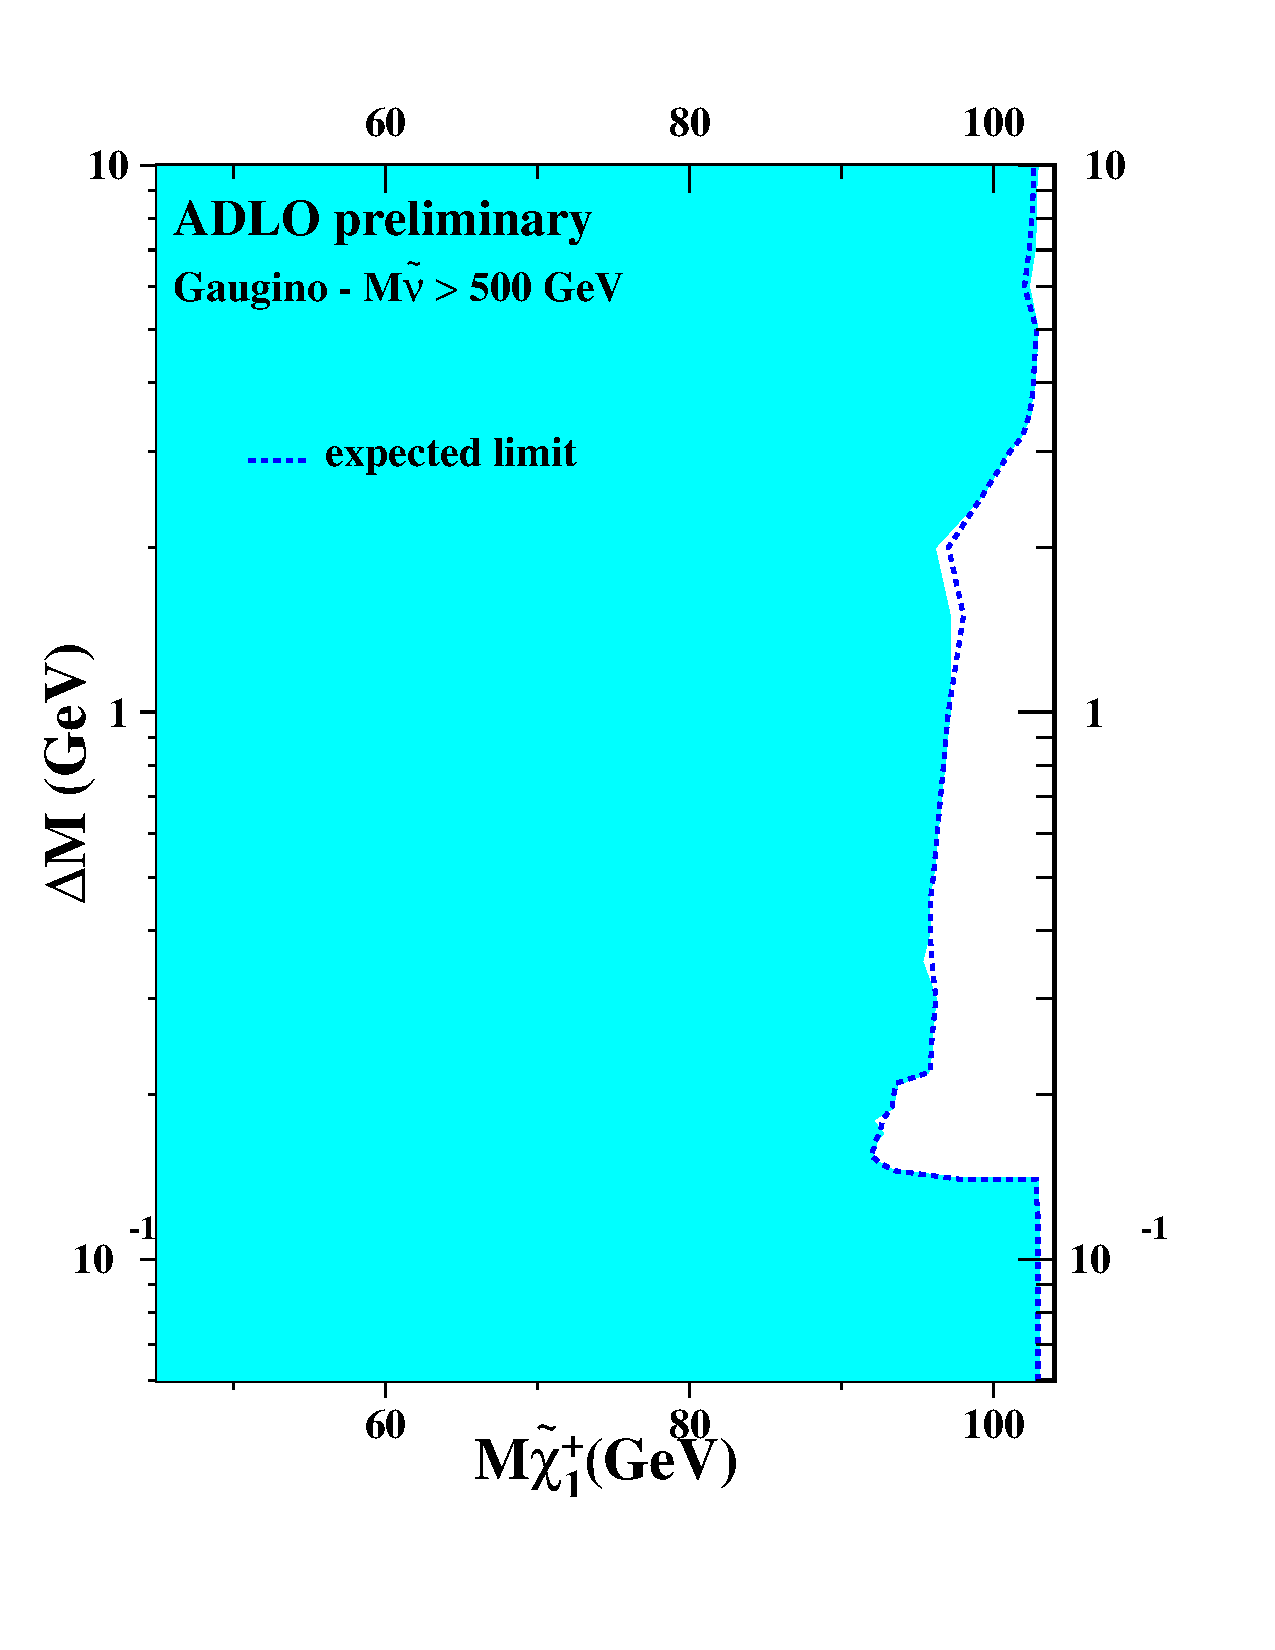
\includegraphics[width=0.45\textwidth]{figures/theory/mass_adlo_gaug_1.pdf}
  \caption{Observed and expected exclusion limits by LEP searches in the $m_{\chipm}-\Delta m \left( \chipm, \chiO \right)$ plane for almost degenerate $M_1$ and $M_2$ and a large unified scalar mass $m_0$. Taken from~\cite{bib:LEP:SUSY_results}.}  
  \label{fig:LEP}
\end{figure}

\subsection*{Searches at ATLAS at 7 and 8\tev}
At the ATLAS experiment at the LHC, searches for events with a disappearing track signature were performed at $\sqrt{s}=7\tev$~\cite{bib:PreviousSearches_Atlas_DT_7TeV} as well as at $\sqrt{s}=8\tev$~\cite{bib:PreviousSearches_Atlas_DT_8TeV}. 
Furthermore, a search for metastable particles with high ionisation losses was performed with $\sqrt{s}=8\tev$ data~\cite{bib:PreviousSearches_ATLAS_DEDX}.
These searches were interpreted within an anomaly-mediated supersymmetry breaking model~\cite{bib:Theory_AMSB_1998} with $\tan\beta=5$ and $\mu>0$.
The excluded parameter space by these searches is shown in Fig.~\ref{fig:ATLAS}.
Models with charginos down to lifetimes of 0.06\ns could be excluded.

\begin{figure}[!b]
  \centering
      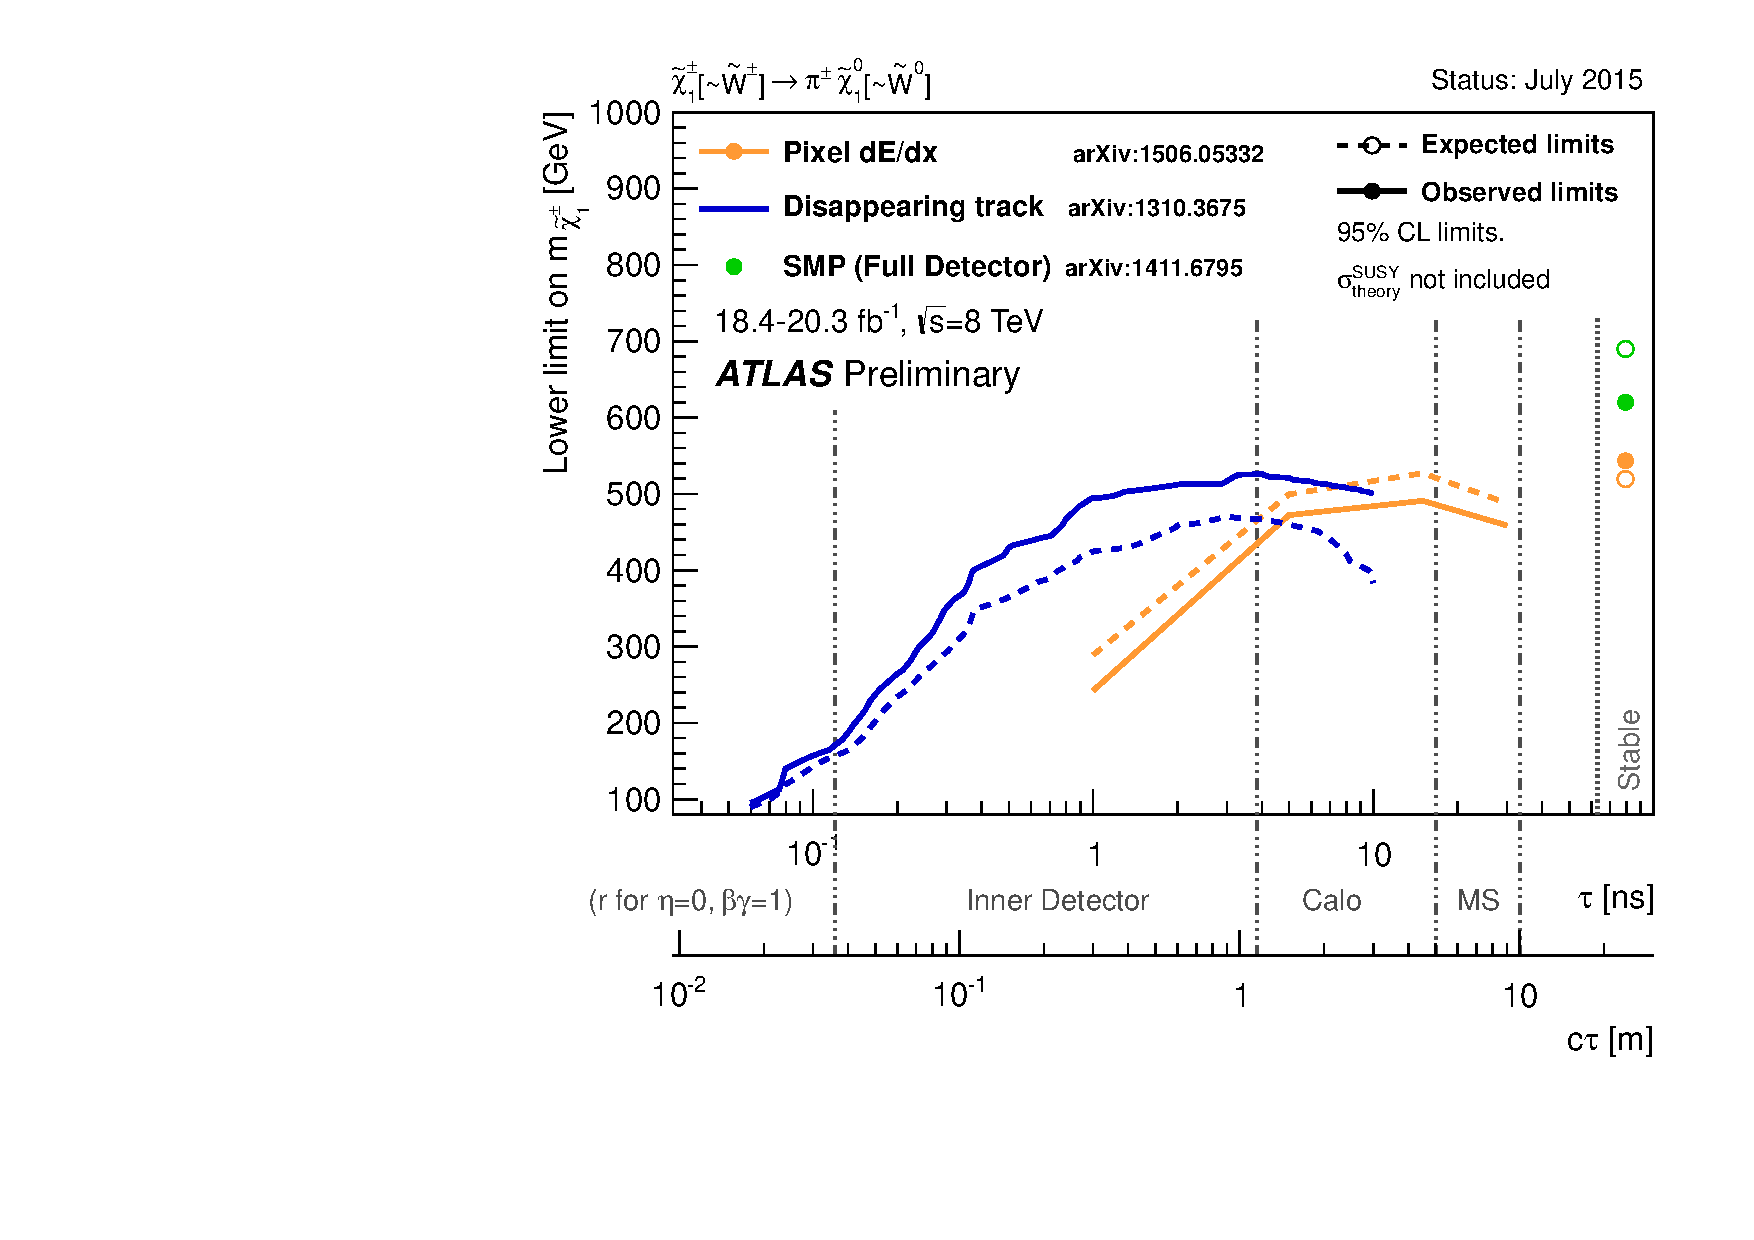
\includegraphics[width=0.54\textwidth]{figures/theory/ATLAS_SUSY_LLPChargino.pdf}
  \caption{Excluded parameter space by ATLAS searches in the $m_{\chipm}-\tau_{\chipm}$ plane for an AMSB model with $\tan\beta=5$ and $\mu>0$. Only chargino pair production is taken into account. The area below the curves is excluded. Taken from~\cite{bib:ATLAS_SUMMARYPLOTS}.}  
  \label{fig:ATLAS}
\end{figure}

\subsection*{Searches at CMS at 7 and 8\tev}
There are several searches at the CMS experiment at the LHC that are sensitive to long-lived wino-like charginos.
Among them is the search for long-lived charged particles~\cite{bib:CMS:HSCP_8TeV}, which searched for heavy particles with large energy deposits in the tracker at $\sqrt{s}=7\tev$  and $\sqrt{s}=8\tev$.
Furthermore, there is the search for disappearing tracks~\cite{bib:CMS:DT_8TeV} which analysed events with disappearing tracks in the tracker with respect to wino-like charginos almost mass-degenerate with the lightest neutralino.
This search was performed at the CMS experiment at a centre-of mass energy of $\sqrt{s}=8\tev$.
Since the latter search is more sensitive to shorter lifetime, only the exclusion limits derived by this search are shown in Fig.~\ref{fig:CMS}.
The disappearing track search by CMS shows a very similar sensitivity as the searches done at the ATLAS experiment.

\begin{figure}[!t]
  \centering
      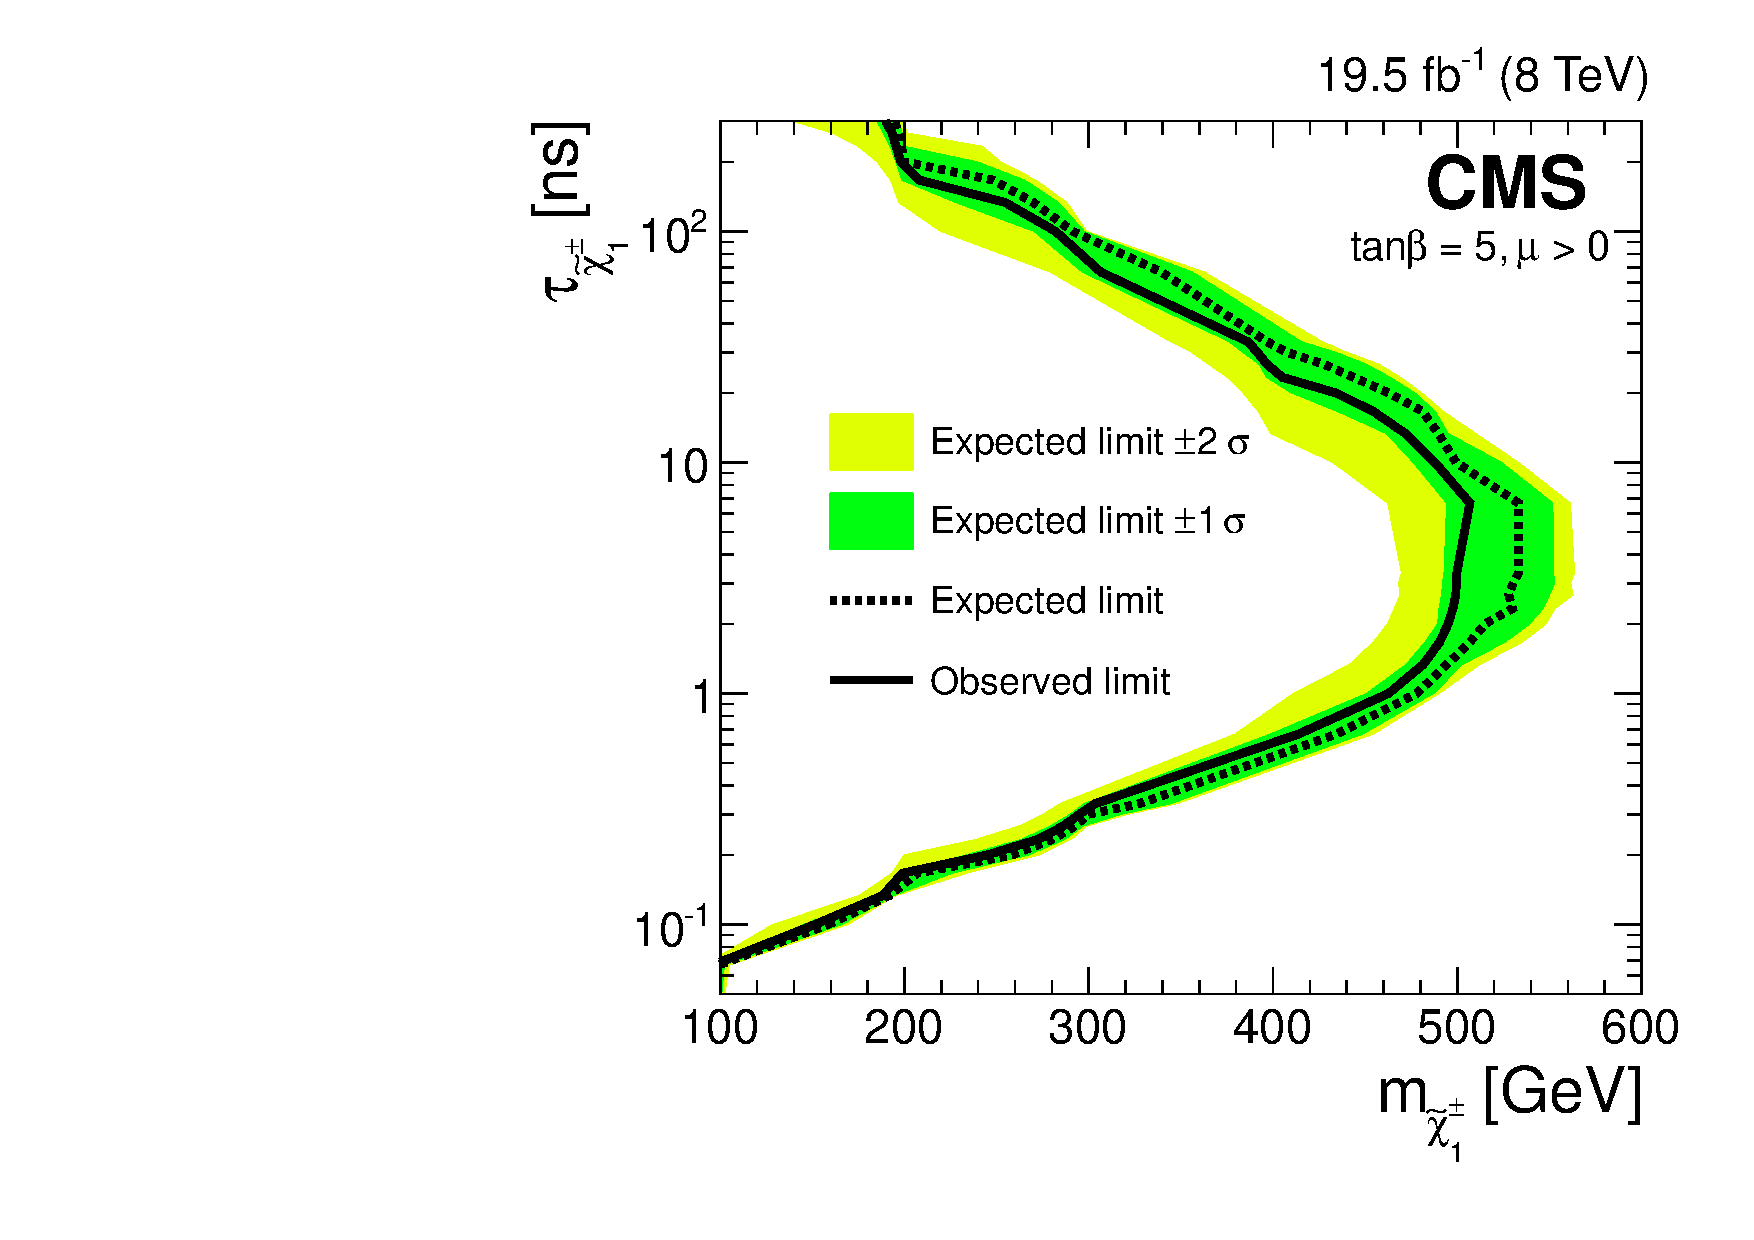
\includegraphics[width=0.54\textwidth]{figures/theory/lifetimeNs_vs_mass.pdf}
  \caption{Excluded parameter space by the Disappearing track search of CMS in the $\tau_{\chipm}-m_{\chipm}$ plane for wino-like charginos. The region left to the curve is excluded. Taken from~\cite{bib:CMS:DT_8TeV}.}  
  \label{fig:CMS}
\end{figure}

\subsection*{Indirect searches}
Finally, also results from indirect Dark Matter searches constrain the parameter region of SUSY models with wino-like charginos and neutralinos.
The most stringent limits are due to results by the Fermi Gamma-Ray Space Telescope (Fermi)~\cite{bib:Fermi} and the High Energy Spectroscopic System (H.E.S.S.)~\cite{bib:HESS}.

By the comparison of the observed gamma-ray signal to the theoretical prediction, Fermi sets upper limits on the Dark Matter annihilation cross-section considering six different decay channels~\cite{bib:Fermi_DM}.

H.E.S.S. sets upper limits on the DM annihilation cross section by the observation of the $\gamma$-ray line which is expected near the DM mass~\cite{bib:HESS_DM}.

Recent interpretations of the Fermi and H.E.S.S. data~\cite{bib:IndirectSearches_Fan_2013,bib:IndirectSearches_Cohen_2013,bib:IndirectSearches_Hryczuk_2014,bib:IndirectSearches_Beneke_2015} show that thermally produced wino-like neutralinos can only account for the full relic density for $\sim3.1\tev$~\cite{bib:IndirectSearches_Cohen_2013}, while DM masses between $1.6-3.0\tev$ are excluded by Fermi and H.E.S.S. observations.
Lower masses are still allowed, however, the neutralino cannot make up the full relic density.
%For scenarios with non-thermally produced neutralinos, the full mass region up to 3.1\tev is ruled out for scenarios where the wino-like neutralino is the only source of Dark Matter~\cite{bib:IndirectSearches_Cohen_2013}. 


